\documentclass[aspectratio=169]{beamer}
\usetheme{Madrid}
\usecolortheme{default}
\usepackage[utf8]{inputenc}
\usepackage[T5]{fontenc}
\usepackage{graphicx}
\usepackage{hyperref}
\usepackage{booktabs}
\usepackage{amsmath}
\usepackage{listings}
\usepackage{xcolor}

\setbeamertemplate{caption}[numbered]
\renewcommand{\figurename}{Hình}
\renewcommand{\thefigure}{10.\arabic{figure}}

% Cấu hình listings cho Python
\definecolor{codegreen}{rgb}{0,0.6,0}
\definecolor{codegray}{rgb}{0.5,0.5,0.5}
\definecolor{codepurple}{rgb}{0.58,0,0.82}
\definecolor{backcolour}{rgb}{0.95,0.95,0.92}

\lstdefinestyle{mystyle}{
    backgroundcolor=\color{backcolour},   
    commentstyle=\color{codegreen},
    keywordstyle=\color{magenta},
    numberstyle=\tiny\color{codegray},
    stringstyle=\color{codepurple},
    basicstyle=\ttfamily\scriptsize,
    breakatwhitespace=false,         
    breaklines=true,                 
    captionpos=b,                    
    keepspaces=true,                 
    numbers=left,                    
    numbersep=5pt,                  
    showspaces=false,                
    showstringspaces=false,
    showtabs=false,                  
    tabsize=2
}
\lstset{style=mystyle}

\title[Chương 10: Trực quan hóa ConvNets]{Học Sâu (Deep Learning) \\ \vspace{0.5cm} \Large Chương 10: Diễn dịch và Trực quan hóa Mạng Tích chập \\ (Interpreting what ConvNets learn)}
\author{Đại học Đông Á}
\date{\today}

\begin{document}

\begin{frame}
    \titlepage
\end{frame}

\begin{frame}{Nội dung chương}
    \tableofcontents
\end{frame}

\section{1. Vấn đề "Hộp Đen" trong Deep Learning}

\begin{frame}{Deep Learning có phải là Hộp Đen (Black Box)?}
    \begin{itemize}
        \item Định kiến phổ biến cho rằng Mạng nơ-ron là những chiếc "Hộp đen", không thể giải thích được lý do nó đưa ra quyết định (Black Box Problem).
        \item Khả năng diễn dịch (\textbf{Interpretability}) là yêu cầu bắt buộc trong các lĩnh vực rủi ro cao:
        \begin{itemize}
            \item \textbf{Y tế:} "Tại sao AI lại chẩn đoán bệnh nhân này bị ung thư?"
            \item \textbf{Xe tự lái:} "Tại sao AI lại không nhận ra chiếc xe tải phía trước?"
        \end{itemize}
        \item Thực tế: Định kiến "Hộp đen" \textbf{KHÔNG} đúng với Mạng Tích chập (ConvNets).
        \item ConvNets học các biểu diễn hình ảnh không gian 2D, do đó chúng ta có thể \textbf{trực quan hóa} những gì nó đang "nhìn" thấy.
    \end{itemize}
\end{frame}

\begin{frame}{Các phương pháp Trực quan hóa ConvNet}
    Trong chương này, chúng ta sẽ khảo sát 3 phương pháp cốt lõi nhất để mở khóa hộp đen ConvNet:
    \begin{enumerate}
        \item \textbf{Trực quan hóa Bản đồ đặc trưng trung gian (Intermediate Activations):} Giúp ta hiểu mô hình đang "nhìn" thấy những chi tiết nào của ảnh.
        \item \textbf{Trực quan hóa Bộ lọc (Filter Visualization):} Sử dụng Gradient Ascent để vẽ ra các mẫu họa tiết (Pattern) lý tưởng mà mỗi Bộ lọc khát khao tìm kiếm nhất.
        \item \textbf{Bản đồ Kích hoạt Lớp (Grad-CAM):} Trả lời câu hỏi "Tại sao AI đưa ra quyết định phân loại này?" thông qua một Bản đồ nhiệt (Heatmap) chỉ thẳng vào vùng ảnh quan trọng.
    \end{enumerate}
\end{frame}

\section{2. Trực quan hóa Biểu diễn Trung gian}

\begin{frame}{Kỹ thuật 1: Trực quan hóa Bản đồ Đặc trưng (Feature Maps)}
    \begin{itemize}
        \item \textbf{Mục tiêu:} Hiểu cách các lớp Tích chập liên tiếp (Successive Layers) biến đổi và bóc tách một hình ảnh đầu vào.
        \item \textbf{Khái niệm Kích hoạt (Activations):} Đầu ra của một lớp Tích chập (bao gồm cả chiều không gian $H, W$ và số kênh $C$) được gọi là Activation.
        \item Mỗi kênh (Channel) trong bản đồ đặc trưng hoạt động như một bộ dò mẫu (Pattern Detector) tương đối độc lập. Do đó ta sẽ xuất hình ảnh của từng Kênh ra màn hình để phân tích.
    \end{itemize}
\end{frame}

\begin{frame}{Ví dụ Đầu vào}
    \begin{columns}
        \column{0.5\textwidth}
        \begin{itemize}
            \item Ta đưa một bức ảnh con mèo (hoàn toàn mới, không có trong tập huấn luyện) vào mạng CNN phân loại Chó-Mèo đã được train ở Chương 8.
            \item Hãy xem cách các lớp Tích chập phản ứng (Activate) với bức ảnh này.
        \end{itemize}
        
        \column{0.5\textwidth}
        \begin{figure}
            \centering
            
\includegraphics[width=\textwidth,height=0.6\textheight,keepaspectratio]{../../images/ch10/cat.135f6a4b.png}
            \caption{Hình ảnh con mèo thử nghiệm}
        \end{figure}
    \end{columns}
\end{frame}

\begin{frame}[fragile]{Tiền xử lý ảnh gốc}
Chúng ta dùng \texttt{keras.utils} để load ảnh gốc và chuyển nó thành mảng numpy Tensor sẵn sàng đưa vào mô hình.

\begin{lstlisting}[language=Python]
import keras
import numpy as np
import matplotlib.pyplot as plt

img_path = "cat.jpg"
def get_img_array(img_path, target_size):
    # Opens the image file and resizes it
    img = keras.utils.load_img(img_path, target_size=target_size)
    # Turns the image into a float32 NumPy array
    array = keras.utils.img_to_array(img)
    # We add a dimension to transform our array into a "batch"
    array = np.expand_dims(array, axis=0)
    return array

img_tensor = get_img_array(img_path, target_size=(180, 180))
\end{lstlisting}
\end{frame}

\begin{frame}[fragile]{Xây dựng Mô hình Đa Đầu ra (Multi-output Model)}
Để trích xuất các bản đồ đặc trưng ở giữa mạng (Intermediate), ta phải định nghĩa một Model đặc biệt nhận 1 đầu vào nhưng xuất ra \textbf{nhiều đầu ra} tương ứng với mọi lớp Conv2D.

\begin{lstlisting}[language=Python]
from keras import layers

layer_outputs = []
layer_names = []
# Extracts the outputs of all Conv2D and MaxPooling2D layers
for layer in model.layers:
    if isinstance(layer, (layers.Conv2D, layers.MaxPooling2D)):
        layer_outputs.append(layer.output)
        layer_names.append(layer.name)

# Creates a model that will return these outputs
activation_model = keras.Model(inputs=model.input, outputs=layer_outputs)

# Returns a list of nine NumPy arrays 
activations = activation_model.predict(img_tensor)
\end{lstlisting}
\end{frame}

\begin{frame}{Kích hoạt của các Bộ lọc Đơn lẻ (Single Filter)}
    \begin{columns}
        \column{0.5\textwidth}
        \begin{itemize}
            \item Quan sát một kênh ở \textbf{Lớp đầu tiên} của mô hình. Kích thước Tensor: \texttt{(1, 178, 178, 32)}.
            \item Lớp này giữ lại gần như toàn bộ thông tin không gian chi tiết của con mèo.
            \item Kênh này đang hoạt động như một công cụ \textbf{Dò tìm Cạnh (Edge Detector)}, cực kỳ nhạy cảm với các đường viền nghiêng.
        \end{itemize}
        
        \column{0.5\textwidth}
        \begin{figure}
            \centering
            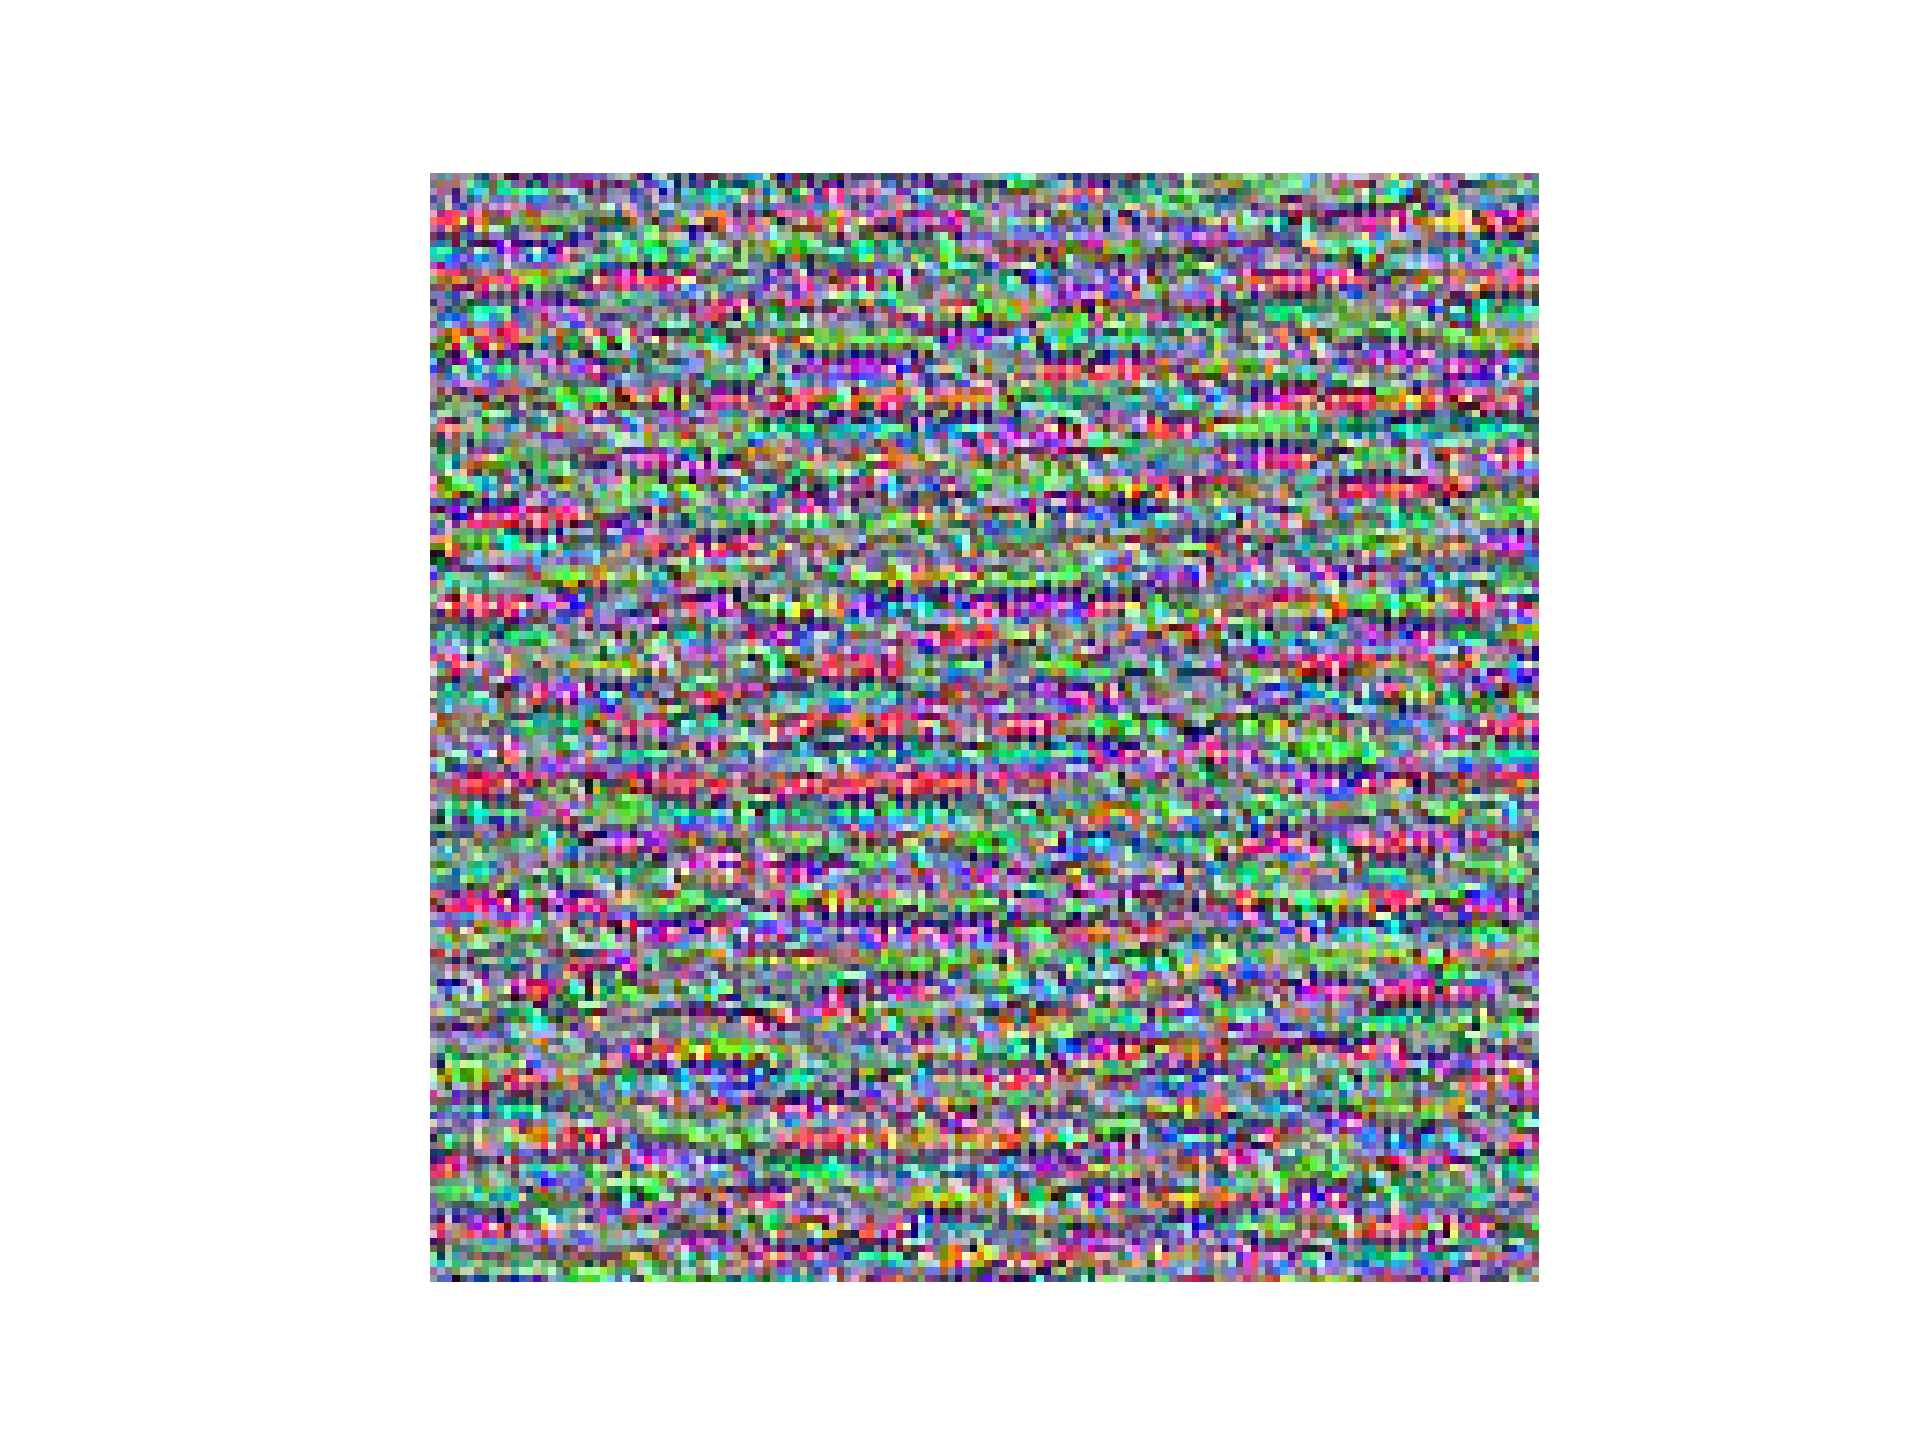
\includegraphics[width=\textwidth,height=0.7\textheight,keepaspectratio]{../../images/ch10/single_filter.8d2772d6.png}
            \caption{Đặc trưng Kênh số 4 (Lớp Conv đầu tiên)}
        \end{figure}
    \end{columns}
\end{frame}

\begin{frame}{Kích hoạt Kênh đặc biệt (Mắt mèo)}
    \begin{columns}
        \column{0.5\textwidth}
        \begin{itemize}
            \item Một kênh khác ở cùng lớp đầu tiên lại có nhiệm vụ hoàn toàn khác.
            \item Kênh số 5 này đặc biệt nhạy cảm với những \textbf{đốm sáng hình tròn} (như con ngươi của mắt mèo) và bỏ qua hầu hết các thông tin về lông hoặc cạnh tai.
            \item Quá trình chuyên môn hóa của các nơ-ron đã bắt đầu ngay từ lớp nông nhất.
        \end{itemize}
        
        \column{0.5\textwidth}
        \begin{figure}
            \centering
            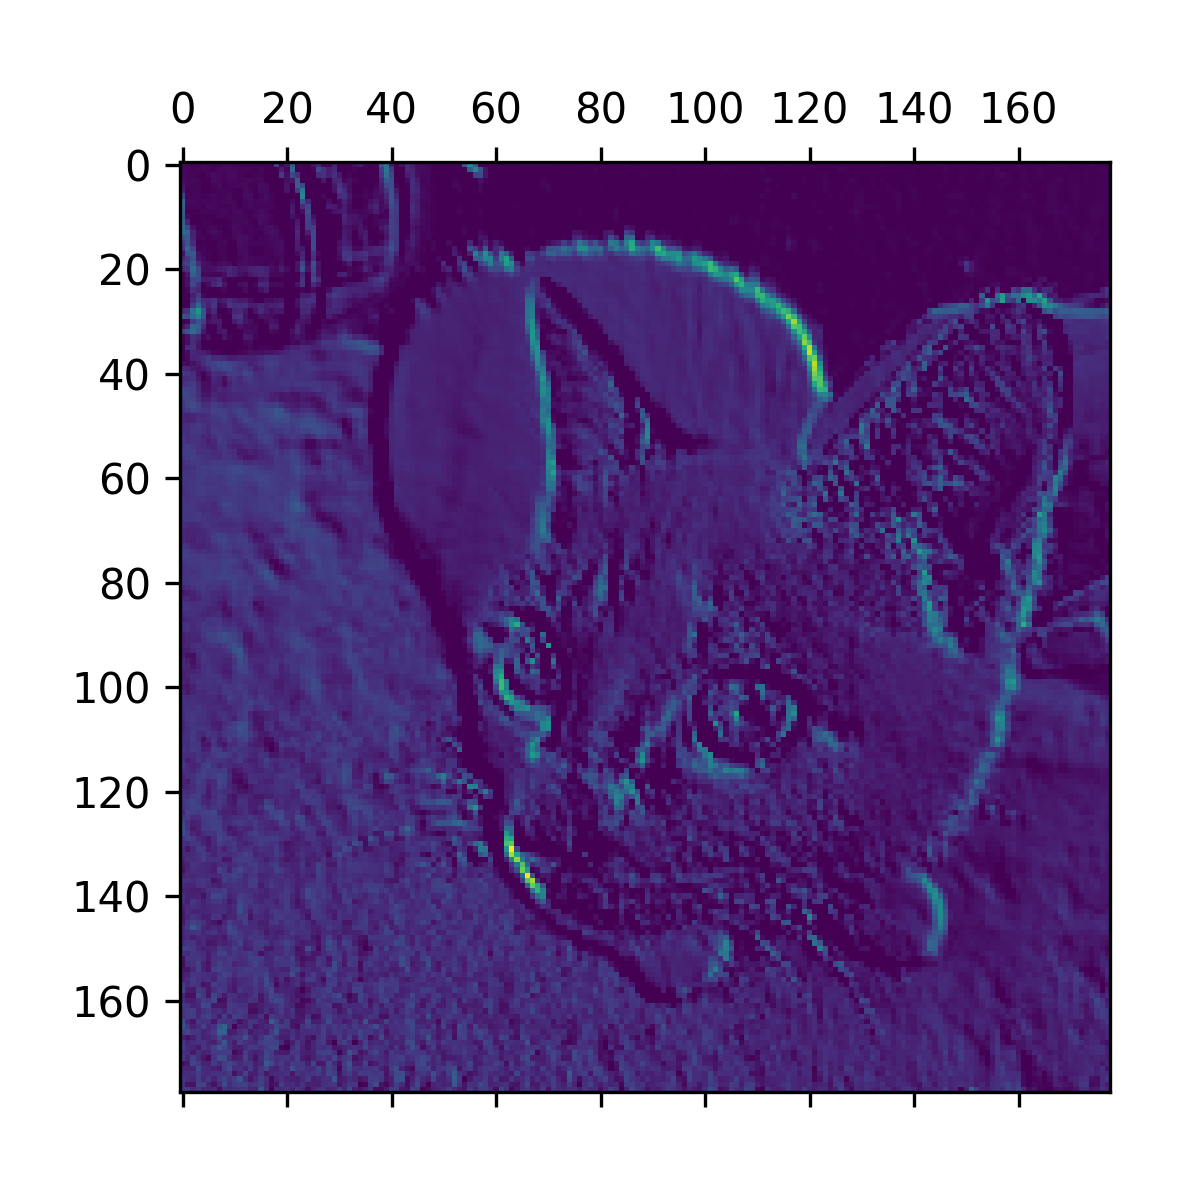
\includegraphics[width=\textwidth,height=0.7\textheight,keepaspectratio]{../../images/ch10/fifth_activation.3dac2691.png}
            \caption{Đặc trưng Kênh số 5 (Bắt dính Mắt mèo)}
        \end{figure}
    \end{columns}
\end{frame}

\begin{frame}[fragile]{Trực quan hóa Toàn bộ Các kênh của Mạng (Phần 1)}
Viết một vòng lặp \texttt{for} lồng nhau để lấy từng kênh ra và vẽ thành một lưới (Grid) ma trận lớn.

\begin{lstlisting}[language=Python]
images_per_row = 16
for layer_name, layer_activation in zip(layer_names, activations):
    n_features = layer_activation.shape[-1]
    size = layer_activation.shape[1]
    n_cols = n_features // images_per_row
    display_grid = np.zeros(
        ((size + 1) * n_cols - 1, images_per_row * (size + 1) - 1)
    )
    for col in range(n_cols):
        for row in range(images_per_row):
            channel_index = col * images_per_row + row
            channel_image = layer_activation[0, :, :, channel_index].copy()
\end{lstlisting}
\end{frame}

\begin{frame}[fragile]{Trực quan hóa Toàn bộ Các kênh của Mạng (Phần 2)}
Ta cần Normalize giá trị của từng channel về phổ màu $0-255$ để màn hình máy tính có thể render được.

\begin{lstlisting}[language=Python]
            # Normalizes channel values within the [0, 255] range.
            if channel_image.sum() != 0:
                channel_image -= channel_image.mean()
                channel_image /= channel_image.std()
                channel_image *= 64
                channel_image += 128
            channel_image = np.clip(channel_image, 0, 255).astype("uint8")
            
            # Places the channel matrix in the empty grid
            display_grid[
                col * (size + 1) : (col + 1) * size + col,
                row * (size + 1) : (row + 1) * size + row,
            ] = channel_image
\end{lstlisting}
\end{frame}

\begin{frame}{Mạng Tích chập học được gì? (Lưới Kích hoạt)}
    \begin{columns}
        \column{0.5\textwidth}
        \begin{itemize}
            \item Khi tiến sâu hơn vào mạng, các bản đồ đặc trưng trở nên \textbf{thưa thớt (Sparse)} và \textbf{trừu tượng (Abstract)}.
            \item Chúng không còn chứa hình dáng vật lý của con mèo nữa, mà chuyển sang lưu giữ các Khái niệm (Ví dụ: "Có tai mèo trong vùng không gian này hay không?").
            \item Các ô trống đen xì nghĩa là bộ lọc đó hoàn toàn không tìm thấy mẫu mà nó cần.
        \end{itemize}
        
        \column{0.5\textwidth}
        \begin{figure}
            \centering
            \includegraphics[width=\textwidth,height=0.8\textheight,keepaspectratio]{../../images/ch10/all_activations.7a8d82cd.png}
            \caption{Kích hoạt của toàn bộ các tầng trong mô hình}
        \end{figure}
    \end{columns}
\end{frame}

\begin{frame}{Sự chưng cất thông tin (Information Distillation)}
    \begin{itemize}
        \item Chúng ta vừa quan sát một hiện tượng phổ quát của Deep Learning: \textbf{Các tầng sâu sẽ học các đặc trưng trừu tượng hơn}.
        \item Mạng AI hoạt động như một \textbf{Ống chưng cất thông tin} (Information Distillation Pipeline).
        \item Các thông tin thừa thãi mang tính tiểu tiết (màu sắc lông, nền tường) sẽ bị lặp tức gạt bỏ. Những thông tin sống còn mang tính phân loại (có tai nhọn, có ria mép) sẽ được phóng đại và lưu giữ.
        \item Điều này giống hệt cách não bộ con người hoạt động: Khi nhìn 1 chiếc xe đạp, bạn chỉ nhớ "Đây là xe đạp" chứ không thể nhớ số nan hoa hay màu phanh xe.
    \end{itemize}
\end{frame}

\section{3. Trực quan hóa Bộ lọc bằng Gradient Ascent}

\begin{frame}{Kỹ thuật 2: Gradient Ascent trên Không gian Ảnh}
    \begin{itemize}
        \item \textbf{Mục tiêu:} Thay vì xem Bộ lọc phản ứng với ảnh thật như thế nào, ta hãy \textbf{tự tạo ra một bức ảnh ảo} (từ mảng nhiễu trắng ngẫu nhiên) sao cho Bộ lọc đó phản ứng cực đại.
        \item Bức ảnh ảo sinh ra chính là hiện thân cho "Mẫu lý tưởng" (Ideal Pattern) mà Bộ lọc đó đang khát khao tìm kiếm.
        \item Đây là thuật toán \textbf{Gradient Ascent (Leo đồi Gradient)}, đi ngược lại với Gradient Descent truyền thống.
    \end{itemize}
\end{frame}

\begin{frame}{Toán học của Gradient Ascent trên Pixel}
    Trong huấn luyện thông thường (Gradient Descent): Cố định Dữ liệu, \textbf{Cập nhật Trọng số (Weights)} để giảm thiểu Hàm Loss về cực tiểu.
    \begin{equation}
        W_{new} = W_{old} - \alpha \cdot \nabla_W L(W)
    \end{equation}
    
    Trong Trực quan hóa Bộ lọc (Gradient Ascent): Cố định Trọng số, \textbf{Cập nhật Pixel của Ảnh ($X$)} để \textbf{tối đa hóa} Giá trị Kích hoạt của Bộ lọc (Activation $A$).
    \begin{equation}
        X_{new} = X_{old} + \alpha \cdot \nabla_X A(X)
    \end{equation}
    
    Ta tính Đạo hàm của Đầu ra Bộ lọc theo Đầu vào Ảnh, sau đó cộng thêm đạo hàm đó vào Ảnh để làm nó rõ nét hơn qua từng epoch.
\end{frame}

\begin{frame}[fragile]{Định nghĩa Hàm Mất mát (Loss) cho Bộ lọc}
Ta dùng cấu trúc Xception siêu mạnh để thực hành kỹ thuật này. Hãy định nghĩa một hàm \texttt{compute\_loss} trả về trung bình giá trị kích hoạt của 1 channel.

\begin{lstlisting}[language=Python]
import keras_hub
from keras import ops

model = keras_hub.models.Backbone.from_preset("xception_41_imagenet")
layer = model.get_layer(name="block3_sepconv1")
feature_extractor = keras.Model(inputs=model.input, outputs=layer.output)

def compute_loss(image, filter_index):
    activation = feature_extractor(image)
    # We avoid border artifacts by discarding the first 2 pixels
    filter_activation = activation[:, 2:-2, 2:-2, filter_index]
    # Returns the mean of the activation values for the filter
    return ops.mean(filter_activation)
\end{lstlisting}
\end{frame}

\begin{frame}[fragile]{Vòng lặp Gradient Ascent (TensorFlow)}
Sử dụng \texttt{tf.GradientTape} để tính toán Gradient của Loss theo Image.

\begin{lstlisting}[language=Python]
import tensorflow as tf

@tf.function
def gradient_ascent_step(image, filter_index, learning_rate):
    with tf.GradientTape() as tape:
        # Explicitly watches the image tensor
        tape.watch(image)
        loss = compute_loss(image, filter_index)
        
    # Computes the gradients of the loss with respect to the image
    grads = tape.gradient(loss, image)
    # Applies the "gradient normalization trick"
    grads = ops.normalize(grads)
    # Moves the image a little bit in a direction that activates it
    image += learning_rate * grads
    return image
\end{lstlisting}
\end{frame}

\begin{frame}[fragile]{Khởi tạo Mảng Nhiễu Trắng ban đầu}
Viết vòng lặp lặp lại 30 bước. Tại thời điểm t=0, bức ảnh là một mảng nhiễu trắng vô nghĩa.

\begin{lstlisting}[language=Python]
def generate_filter_pattern(filter_index):
    iterations = 30
    learning_rate = 10.0
    image = keras.random.uniform(
        # Initialize an image tensor with random values centered on 0.5
        minval=0.4, maxval=0.6, shape=(1, 200, 200, 3)
    )
    
    # Repeatedly updates the values of the image tensor
    for i in range(iterations):
        image = gradient_ascent_step(image, filter_index, learning_rate)
        
    return image[0]
\end{lstlisting}
\end{frame}

\begin{frame}[fragile]{Xử lý hậu kỳ ảnh (Deprocess Image)}
Sau vòng lặp 30 bước, ma trận thu được chứa các giá trị float rất dị thường. Ta phải ép nó về khoảng \texttt{0-255} chuẩn RGB.

\begin{lstlisting}[language=Python]
def deprocess_image(image):
    # Normalizes image values
    image -= ops.mean(image)
    image /= ops.std(image)
    image *= 64
    image += 128
    image = ops.clip(image, 0, 255)
    
    # Center crop to avoid border artifacts
    image = image[25:-25, 25:-25, :]
    image = ops.cast(image, dtype="uint8")
    return ops.convert_to_numpy(image)
\end{lstlisting}
\end{frame}

\begin{frame}{Quần thể các Mẫu Đặc trưng lý tưởng}
    \begin{columns}
        \column{0.5\textwidth}
        \begin{itemize}
            \item Kết quả của Gradient Ascent là những họa tiết kỳ ảo giống như ảo giác (Psychedelic).
            \item Các lớp nông (Shallow): Học màu sắc, vân gỗ, sóng nước.
            \item Các lớp giữa (Middle): Học kết cấu phức tạp hơn (chấm bi, sọc vằn, mạng nhện).
        \end{itemize}
        
        \column{0.5\textwidth}
        \begin{figure}
            \centering
            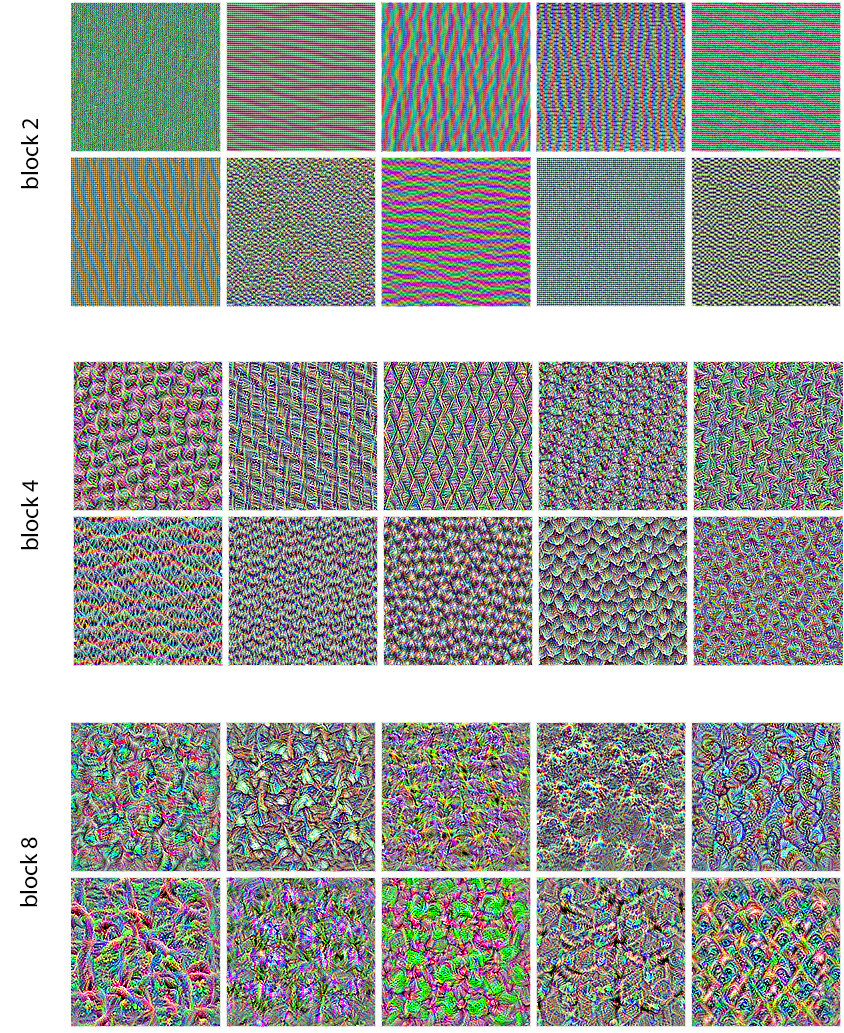
\includegraphics[width=\textwidth,height=0.8\textheight,keepaspectratio]{../../images/ch10/allfilters.8d050d97.png}
            \caption{64 bộ lọc ở các tầng sâu khác nhau}
        \end{figure}
    \end{columns}
\end{frame}

\begin{frame}{Lớp Sâu - Các Khái niệm Đời thực}
    \begin{columns}
        \column{0.5\textwidth}
        \begin{itemize}
            \item Đối với các khối ở cực sâu (như \texttt{block5\_conv1} của VGG16/Xception), các họa tiết bắt đầu mang hình thù của vật thể thực.
            \item Chẳng hạn, bộ lọc này tổng hợp nên họa tiết hình elip đan chéo, rất giống nan hoa xe đạp (Bicycles), lông chim vũ hay vảy bò sát.
            \item Đây là bằng chứng tuyệt vời cho thấy Convolution Layers hoàn toàn có thể hiểu cấu trúc của vạn vật!
        \end{itemize}
        
        \column{0.5\textwidth}
        \begin{figure}
            \centering
            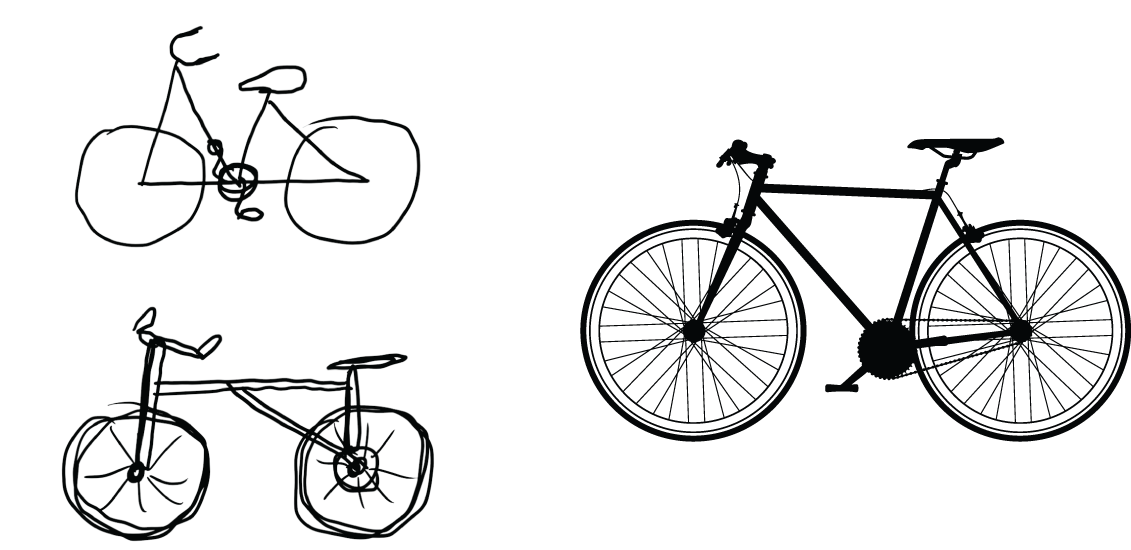
\includegraphics[width=\textwidth,height=0.7\textheight,keepaspectratio]{../../images/ch10/bicycles.c7a8501c.png}
            \caption{Họa tiết bộ lọc siêu sâu (Xe đạp / Vảy)}
        \end{figure}
    \end{columns}
\end{frame}

\section{4. Bản đồ Kích hoạt Lớp (Grad-CAM)}

\begin{frame}{Kỹ thuật 3: Class Activation Map (CAM)}
    \begin{itemize}
        \item \textbf{Mục tiêu:} Trả lời câu hỏi "Phần nào của bức ảnh đã khiến Mạng CNN đưa ra quyết định phân loại này?".
        \item Rất hữu ích cho \textbf{Phân tích lỗi (Error Analysis)} (Tại sao nhận diện sai?) và \textbf{Khám phá Y khoa} (Chỉ ra khối u nằm ở đâu trên ảnh X-Quang phổi).
        \item Phương pháp SOTA (State-of-the-art) là \textbf{Grad-CAM} (Gradient-weighted Class Activation Mapping).
    \end{itemize}
\end{frame}

\begin{frame}{Toán học của Grad-CAM}
    \begin{enumerate}
        \item Tính Đạo hàm của xác suất Lớp dự đoán (Vd: African elephant $y^c$) theo toàn bộ Bản đồ đặc trưng (Feature Maps $A^k$) ở Lớp Tích chập \textbf{cuối cùng}.
        \item Lấy Trung bình không gian (Global Average Pooling) của Đạo hàm này để ra Trọng số độ quan trọng $\alpha_k^c$ của Kênh $k$:
        \begin{equation}
            \alpha_k^c = \frac{1}{Z} \sum_i \sum_j \frac{\partial y^c}{\partial A_{i,j}^k}
        \end{equation}
        \item Nhân chập Trọng số với Feature Maps tương ứng, rồi bọc qua hàm ReLU (chỉ lấy phần dương - Positive influence):
        \begin{equation}
            L_{\text{Grad-CAM}}^c = \text{ReLU} \left( \sum_k \alpha_k^c A^k \right)
        \end{equation}
    \end{enumerate}
\end{frame}

\begin{frame}{Đầu vào bài toán Phân tích Lỗi}
    \begin{columns}
        \column{0.5\textwidth}
        \begin{itemize}
            \item Ta đưa bức ảnh chụp hai con Voi châu Phi và con cái của chúng vào mô hình Xception chuẩn.
            \item Lớp \texttt{ImageClassifier} dự đoán: Voi châu Phi (African elephant) với xác suất cực cao.
            \item Câu hỏi đặt ra: Nó nhìn vào Voi mẹ hay Voi con để ra quyết định?
        \end{itemize}
        
        \column{0.5\textwidth}
        \begin{figure}
            \centering
            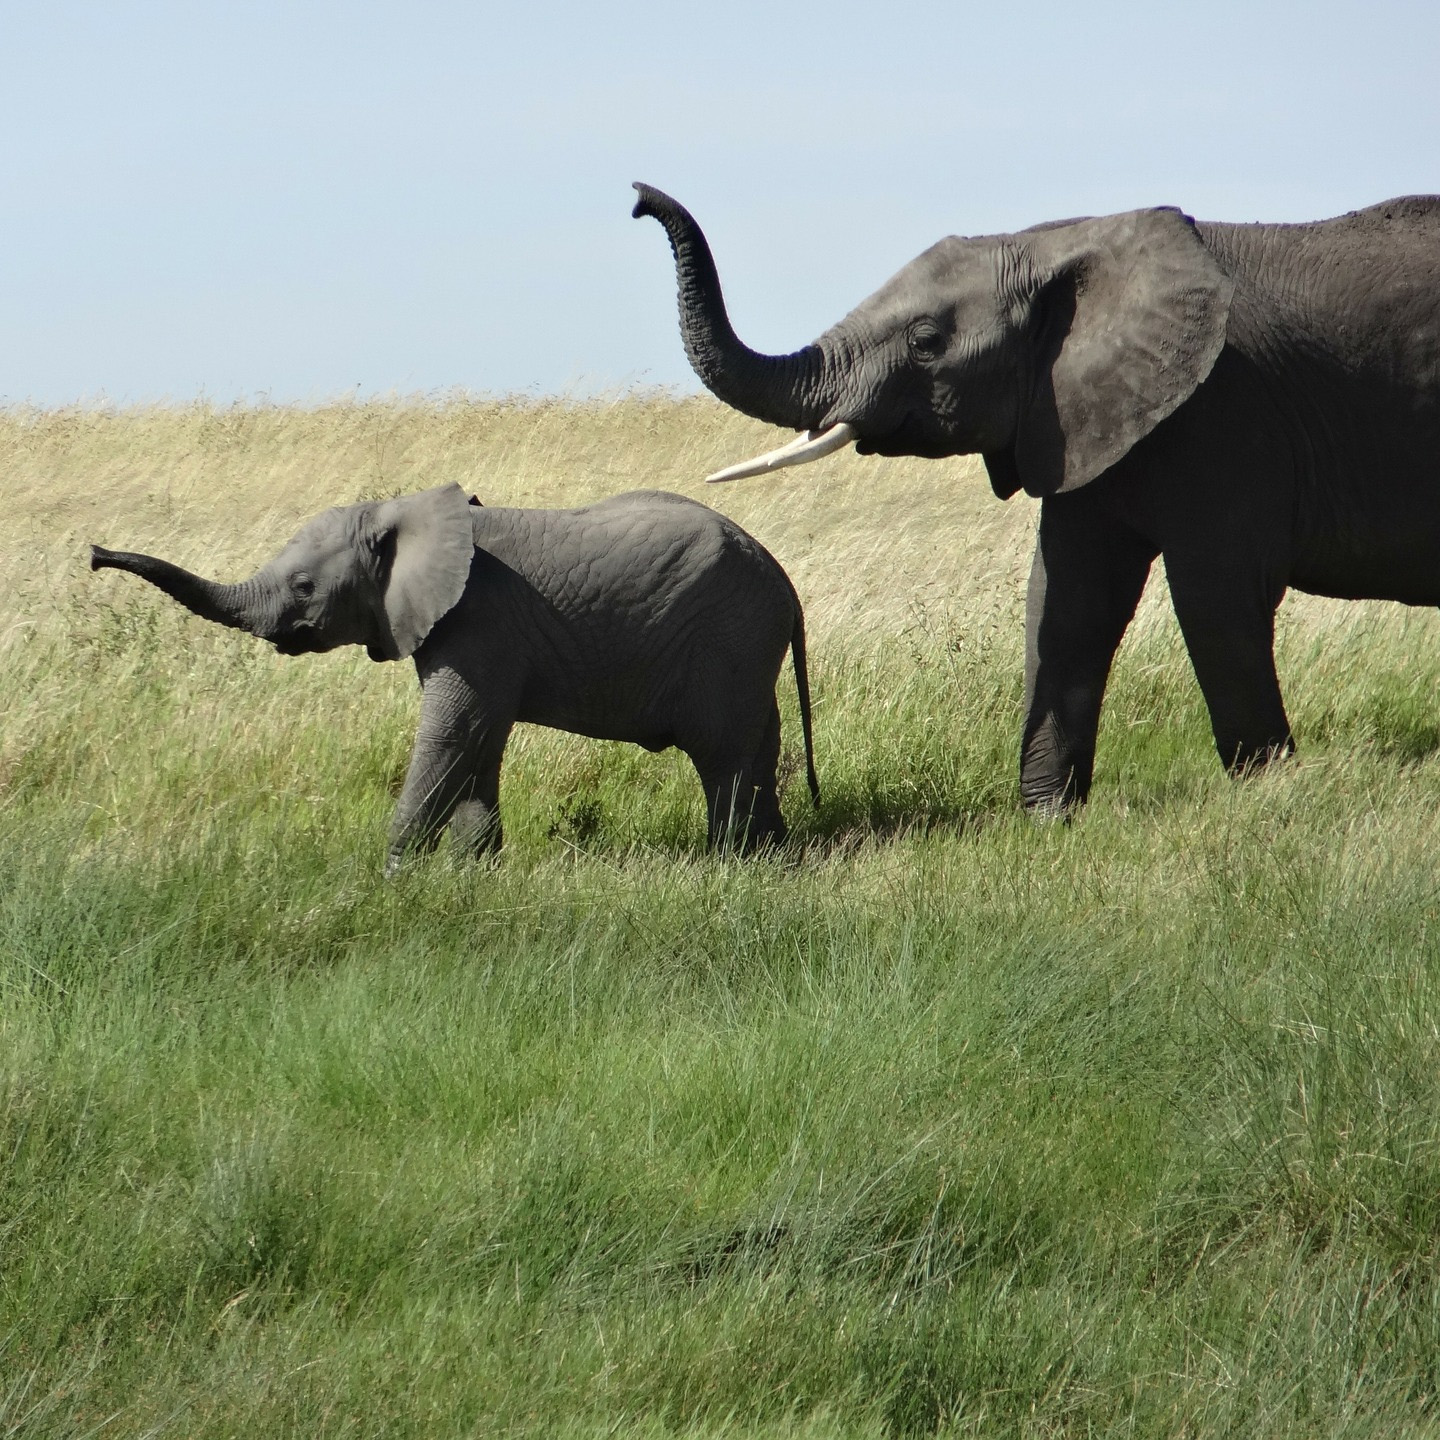
\includegraphics[width=\textwidth,height=0.7\textheight,keepaspectratio]{../../images/ch10/elephant.6abc731a.jpg}
            \caption{Ảnh Voi châu Phi đầu vào}
        \end{figure}
    \end{columns}
\end{frame}

\begin{frame}[fragile]{Chuẩn bị Grad-CAM: Trích xuất Lớp Cuối}
Ta tạo 2 Model phụ: Model 1 lấy đầu ra của Lớp tích chập cuối cùng. Model 2 chạy từ đầu ra đó đến thẳng lớp Softmax dự đoán.

\begin{lstlisting}[language=Python]
# Model 1: From original image to the last conv layer feature map
last_conv_layer_name = "block14_sepconv2_act"
last_conv_layer = model.backbone.get_layer(last_conv_layer_name)
last_conv_layer_model = keras.Model(model.inputs, last_conv_layer.output)

# Model 2: From last conv layer feature map to predictions
classifier_input = last_conv_layer.output
x = classifier_input
for layer_name in ["pooler", "predictions"]:
    x = model.get_layer(layer_name)(x)
classifier_model = keras.Model(classifier_input, x)
\end{lstlisting}
\end{frame}

\begin{frame}[fragile]{Đạo hàm Xếp hạng Lớp (Class Gradients)}
Dùng \texttt{tf.GradientTape} để lấy Gradient của Node dự đoán "African Elephant" đối chiếu với Bản đồ đặc trưng lớp dưới.

\begin{lstlisting}[language=Python]
def get_top_class_gradients(img_array):
    last_conv_layer_output = last_conv_layer_model(img_array)
    with tf.GradientTape() as tape:
        tape.watch(last_conv_layer_output)
        preds = classifier_model(last_conv_layer_output)
        top_pred_index = ops.argmax(preds[0])
        top_class_channel = preds[:, top_pred_index]

    # Gradient of top class w.r.t the feature map
    grads = tape.gradient(top_class_channel, last_conv_layer_output)
    return grads, last_conv_layer_output

grads, last_conv_output = get_top_class_gradients(img_array)
\end{lstlisting}
\end{frame}

\begin{frame}[fragile]{Xây dựng Bản đồ Nhiệt (Heatmap)}
Nhân chập Gradient (Trọng số tầm quan trọng của kênh) vào Feature Map để vẽ ra Heatmap thô.

\begin{lstlisting}[language=Python]
import numpy as np
import matplotlib.pyplot as plt

# Global average pooling the gradients
pooled_grads = np.mean(grads, axis=(0, 1, 2))
last_conv_output = last_conv_output[0].copy()

# Multiplies each channel by how important it is
for i in range(pooled_grads.shape[-1]):
    last_conv_output[:, :, i] *= pooled_grads[i]
    
# The channel-wise mean is our heatmap
heatmap = np.mean(last_conv_output, axis=-1)

# Apply ReLU manually
heatmap = np.maximum(heatmap, 0)
heatmap /= np.max(heatmap)
\end{lstlisting}
\end{frame}

\begin{frame}{Bản đồ Nhiệt thô Grad-CAM}
    \begin{columns}
        \column{0.5\textwidth}
        \begin{itemize}
            \item Kết quả là một mảng Numpy 2D. 
            \item Điểm có giá trị càng cao (Vùng sáng vàng chói) thì càng tác động lớn đến quyết định phân loại "Đây là con voi".
        \end{itemize}
        
        \column{0.5\textwidth}
        \begin{figure}
            \centering
            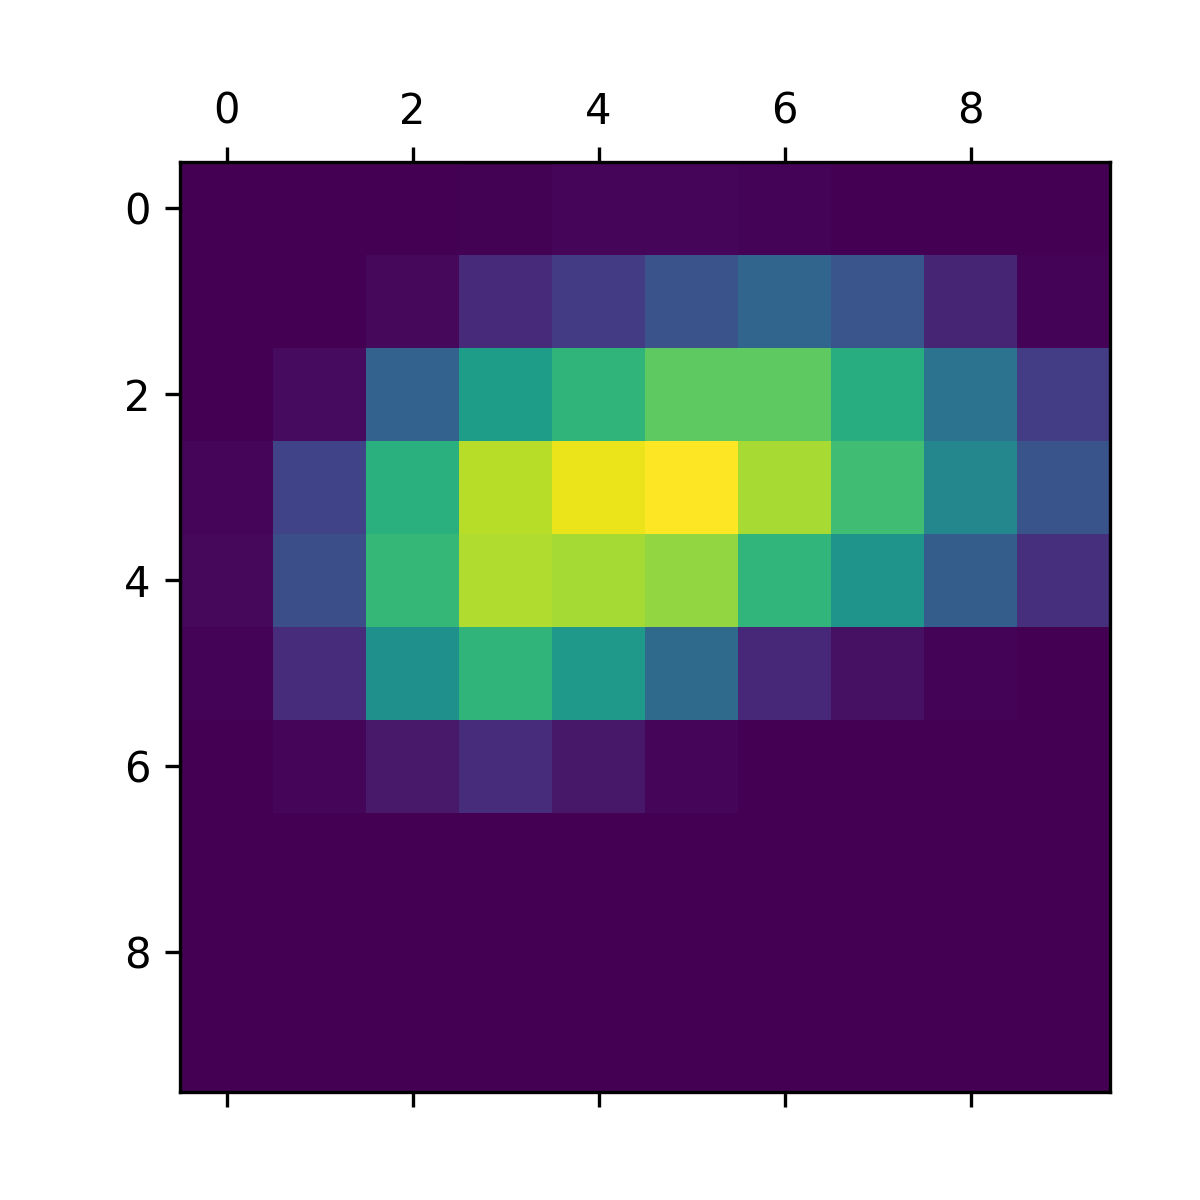
\includegraphics[width=\textwidth,height=0.7\textheight,keepaspectratio]{../../images/ch10/cam.b66fff28.png}
            \caption{Bản đồ nhiệt thô Grad-CAM}
        \end{figure}
    \end{columns}
\end{frame}

\begin{frame}[fragile]{Chồng bản đồ nhiệt (Superimposed Heatmap)}
Ta áp dụng phổ màu JET (Xanh dương sang Đỏ) của \texttt{matplotlib} để nhuộm màu bản đồ, rồi áp lên trên ảnh gốc với hệ số trong suốt $0.4$.

\begin{lstlisting}[language=Python]
import matplotlib.cm as cm

img = keras.utils.load_img(img_path)
img = keras.utils.img_to_array(img)

heatmap = np.uint8(255 * heatmap)
jet = cm.get_cmap("jet")
jet_colors = jet(np.arange(256))[:, :3]
jet_heatmap = jet_colors[heatmap]

jet_heatmap = keras.utils.array_to_img(jet_heatmap)
jet_heatmap = jet_heatmap.resize((img.shape[1], img.shape[0]))
jet_heatmap = keras.utils.img_to_array(jet_heatmap)

# Superimposes the heatmap at 40% opacity
superimposed_img = jet_heatmap * 0.4 + img
\end{lstlisting}
\end{frame}

\begin{frame}{Kết luận về thuật toán định vị trí}
    \begin{columns}
        \column{0.5\textwidth}
        \begin{itemize}
            \item \textbf{Kết luận đột phá:} Vùng đỏ rực tập trung chính xác vào \textbf{Đôi tai} của Voi con. Tai là đặc điểm sinh học định danh duy nhất phân biệt Voi châu Phi và Voi Ấn Độ.
            \item Mạng AI hoàn toàn không bị ngốc! Nó đã học đúng đặc điểm nhận dạng cốt lõi của sinh học phân tử thay vì học lỏm bầu trời hay cành cây.
        \end{itemize}
        
        \column{0.5\textwidth}
        \begin{figure}
            \centering
            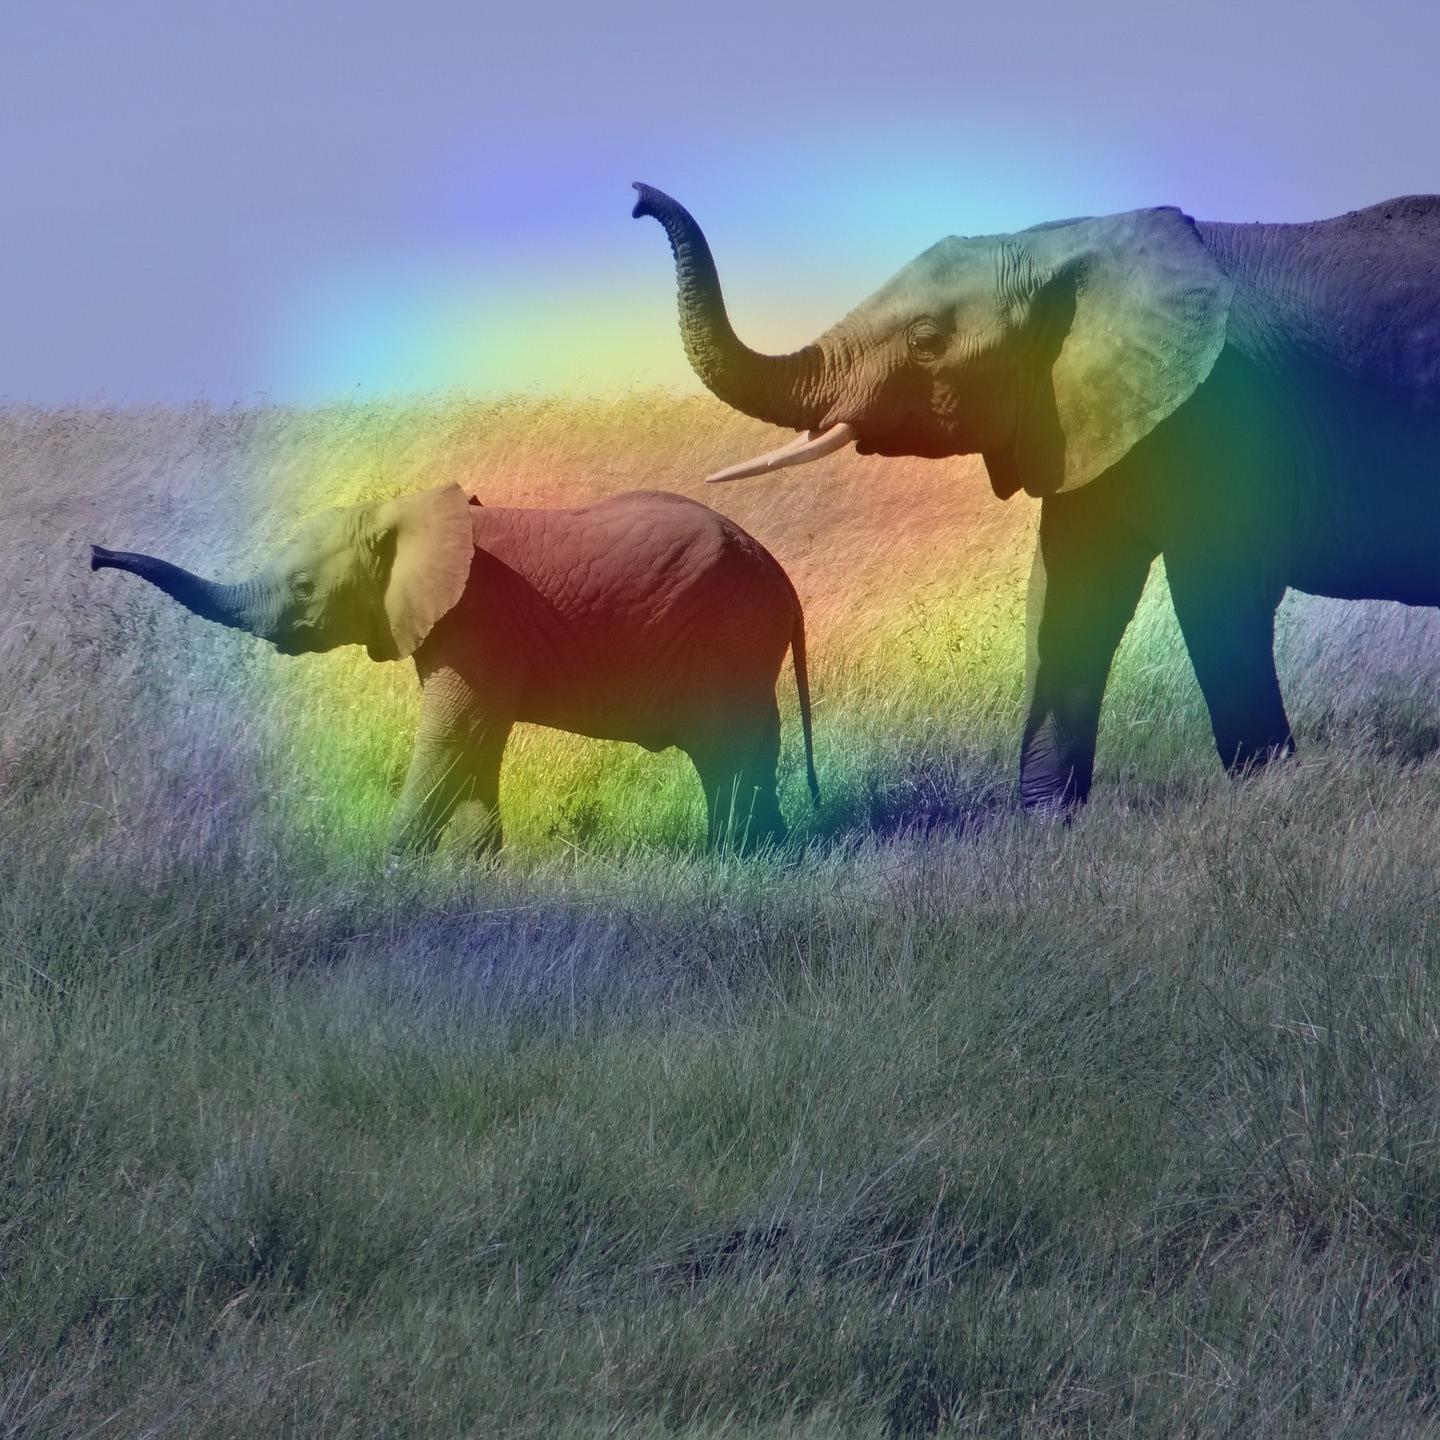
\includegraphics[width=\textwidth,height=0.7\textheight,keepaspectratio]{../../images/ch10/elephant_cam.73b7f8e0.jpg}
            \caption{Bản đồ Grad-CAM hiển thị tai Voi con}
        \end{figure}
    \end{columns}
\end{frame}

\section{Tổng kết}

\begin{frame}{Tổng kết Chương 10}
    \begin{itemize}
        \item Mạng Tích chập \textbf{KHÔNG} phải là Hộp đen. Ta hoàn toàn có thể "Nội soi" chúng dễ dàng bằng ngôn ngữ Python.
        \item \textbf{Intermediate Activations:} Phân tích tính trừu tượng tăng dần của Feature Maps (từ cạnh, góc đến mắt mèo).
        \item \textbf{Filter Visualization (Gradient Ascent):} Đạo hàm ngược lên Pixel ảnh để sinh ra ảnh ảo giác nhằm hiểu xem mỗi Bộ lọc khát khao tìm kiếm họa tiết nào.
        \item \textbf{Grad-CAM (Bản đồ Kích hoạt Lớp):} Trích xuất Heatmap vùng màu Đỏ để xác định vùng quyết định đóng góp lớn nhất vào Output dự đoán, là công cụ không thể thiếu trong X-Quang y tế học sâu.
    \end{itemize}
\end{frame}

\end{document}
